\chapter{Fourier Transform}
\begin{enumerate}
	\item Let $F(k)$ is the Fourier exponential transform of $f(x)$ and $G(k)$ be the Fourier Transform of $g(x)=f(x+a)$. Then $G(k)$ is given by
	(Use the Fourier integral $F(k)=\frac{1}{\sqrt{2 \pi}} \int_{-\infty}^{+\infty} f(x) e^{i k x} d x$ )
	 \begin{tasks}(2)
		\task[\textbf{a.}]$e^{i a k} f(k)$
		\task[\textbf{b.}]$e^{-i a k} F(-k)$
		\task[\textbf{c.}] $e^{-i a k} F(k)$
		\task[\textbf{d.}] $e^{-i a k} f(k)$
	\end{tasks}
	\item The value of a function is given by $f(x)=\left\{\begin{array}{cc}1 & 0<x<1 \\ -1 & 1<x<2 \\ 0 & x>2\end{array}\right.$, the Fourier cosine transform of $f(x)$ is
	 \begin{tasks}(2)
		\task[\textbf{a.}]$\sqrt{\frac{2}{\pi}}\left(\frac{2 \sin \omega+\sin 2 \omega}{\omega}\right)$
		\task[\textbf{b.}]$\sqrt{\frac{2}{\pi}}\left(\frac{2 \sin \omega-\sin 2 \omega}{\omega}\right)$
		\task[\textbf{c.}]$\sqrt{\frac{2}{\pi}}\left(\frac{\sin \omega-\sin 2 \omega}{\omega}\right)$
		\task[\textbf{d.}] $\sqrt{\frac{2}{\pi}}\left(\frac{2 \sin \omega}{\omega}\right)$
	\end{tasks}
	\item Consider the function $\delta_{n}(x)=\frac{n}{\sqrt{\pi}} \exp \left(-n^{2} x^{2}\right)$. For $n \rightarrow \infty$ The Fourier transform of the function is given by
	 \begin{tasks}(2)
		\task[\textbf{a.}]$\delta(x)=\int_{-\infty}^{+\infty} e^{-i k x} d k$
		\task[\textbf{b.}]$\delta(x)=\frac{1}{2 \pi} \int_{-\infty}^{+\infty} e^{i k x} d k$
		\task[\textbf{c.}]$\delta(x)=\frac{1}{2 \pi} \int_{-\infty}^{+\infty} e^{-i k x} d k$
		\task[\textbf{d.}] 0
	\end{tasks}
	\item For the function $f(t)=\delta(t-x)$, the Fourier cosine integral is defined as $g_{c}(\omega)=\sqrt{\frac{2}{\pi}} \int_{0}^{\infty} f(t) \cos \omega t d t$. Its Fourier transform is:
	 \begin{tasks}(2)
		\task[\textbf{a.}] $\sqrt{\frac{2}{\pi}} \cos \omega x$
		\task[\textbf{b.}]$\sqrt{\frac{2}{\pi}}$
		\task[\textbf{c.}]$\sqrt{\frac{2}{\pi}} \sin \omega x$
		\task[\textbf{d.}] $i \sqrt{\frac{2}{\pi}}$
	\end{tasks}
	\item Inverse cosine transform of $g_{c}(\omega)=\sqrt{\frac{2}{\pi}} \cos \omega x$ is:
	 \begin{tasks}(2)
		\task[\textbf{a.}]$\delta(t+x)$
		\task[\textbf{b.}]$\delta(t-x)$
		\task[\textbf{c.}]$\delta(t-x)(t+x)$
		\task[\textbf{d.}] $\delta^{2}(x-t)(x+t)$
	\end{tasks}
	\item $f(t)=\frac{\hbar}{2 \pi i} \int_{-\infty}^{+\infty} \frac{e^{-i \omega t} d \omega}{\left(E_{0}-i \Gamma / 2-\hbar \omega\right)}$ The value of $f(t)$ is given by
	 \begin{tasks}(2)
		\task[\textbf{a.}](a) $f(t)= \begin{cases}e^{-\Gamma t / 2 \hbar} e^{-i E_{0} t / \hbar} & , t>0 \\ 0 & , t<0\end{cases}$
		\task[\textbf{b.}]$f(t)= \begin{cases}e^{\sqrt{1 / 2 \hbar}} e^{-1 E_{0} t / \hbar} & , t>0 \\ 0 & , t<0\end{cases}$
		\task[\textbf{c.}]$f(t)= \begin{cases}e^{-\Gamma t / 2 \hbar} e^{-i E_{0} t / \hbar} & , t>0 \\ 0 & , t<0\end{cases}$
		\task[\textbf{d.}] $f(t)= \begin{cases}e^{-\Gamma t / 2 h} e^{-i E_{0} t / h} & , t>0 \\ e^{-i E_{0} t / \hbar} & , t<0\end{cases}$
	\end{tasks}
	\item The Fourier transform of function $h(t)=t e^{-t^{2}}$ is 
	 \begin{tasks}(2)
		\task[\textbf{a.}] $j \pi f e^{-\pi^{2} f^{2}}$
		\task[\textbf{b.}]$-j \pi f e^{-\pi^{2} f^{2}}$
		\task[\textbf{c.}]$j \pi f e^{-\pi^{2} f^{2} / 4}$
		\task[\textbf{d.}] $-j \pi f e^{-\pi^{2} f^{2} / 4}$
	\end{tasks}
	\item The graph of a real periodic function $f(x)$ for the range $[-\infty, \infty]$ is shown below
	\begin{figure}[H]
		\centering
		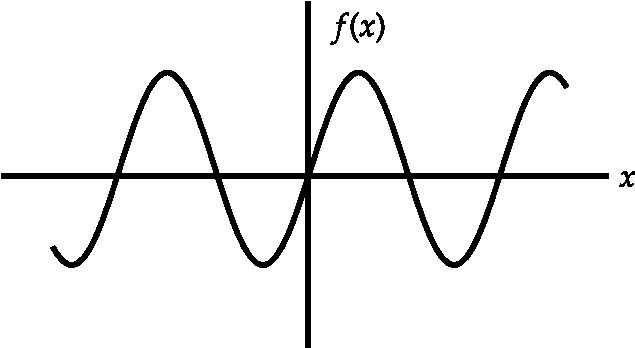
\includegraphics[height=3cm,width=5cm]{FT-Assignment-05}
	\end{figure}
	Which of the following graphs represents the real part of its Fourier transform?
	 \begin{tasks}(2)
		\task[\textbf{a.}]	
		\begin{figure}[H]
			\centering
			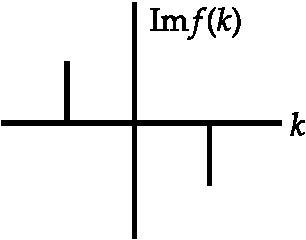
\includegraphics[height=2.2cm,width=3cm]{FT-Assignment-01}
		\end{figure}
		\task[\textbf{b.}]
			\begin{figure}[H]
			\centering
			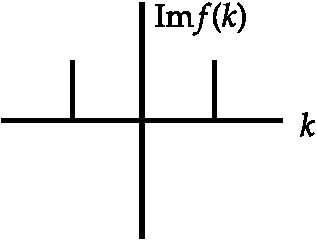
\includegraphics[height=2.2cm,width=3cm]{FT-Assignment-02}
		\end{figure}
		\task[\textbf{c.}]
			\begin{figure}[H]
			\centering
			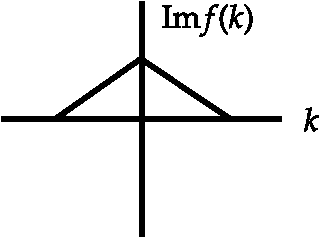
\includegraphics[height=2.2cm,width=3cm]{FT-Assignment-03}
		\end{figure}
		\task[\textbf{d.}] 
			\begin{figure}[H]
			\centering
			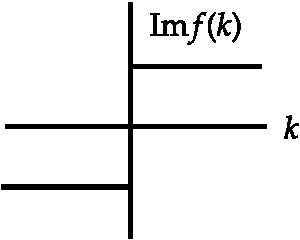
\includegraphics[height=2.2cm,width=3cm]{FT-Assignment-04}
		\end{figure}
	\end{tasks}
	\item The Fourier transform of the function $h(t)=\left\{\begin{array}{cc}\beta e^{-a t}, & t>0 \\ 0, & t<0\end{array}\right.$, is given by
	 \begin{tasks}(2)
		\task[\textbf{a.}]$H(f)=\frac{\alpha}{\sqrt{\alpha^{2}+(2 \pi f)^{2}}} e^{j \tan ^{-1}\left[-2 \pi f^{\prime \alpha]}\right.}$
		\task[\textbf{b.}]$H(f)=\frac{\beta}{\sqrt{\alpha^{2}+(2 \pi f)^{2}}} e^{j \tan ^{-1}[-2 \pi f / \beta]}$
		\task[\textbf{c.}]$H(f)=\frac{\beta}{\sqrt{\alpha^{2}+(2 \pi f)^{2}}} e^{\tan ^{-1}[2 \pi f / \alpha]}$
		\task[\textbf{d.}] $H(f)=\frac{\beta}{\sqrt{\alpha^{2}+(2 \pi f)^{2}}} e^{j \tan ^{-1}[-2 \pi f / \alpha]}$
	\end{tasks}
	\item The Fourier transform of $f(x)=\left\{\begin{array}{cl}-1 & -1<x<0 \\ 1 & 0<x<1 \\ 0 & \text { otherwise }\end{array}\right.$ is
	 \begin{tasks}(2)
		\task[\textbf{a.}] $\frac{i}{\omega} \sqrt{\frac{2}{\pi}}(\cos \omega+1)$
		\task[\textbf{b.}] $\frac{i}{\omega} \sqrt{\frac{2}{\pi}}(\cos \omega-1)$
		\task[\textbf{c.}]$-\frac{i}{\omega} \sqrt{\frac{2}{\pi}}(1+\cos \omega)$
		\task[\textbf{d.}] $\frac{i}{\omega} \sqrt{\frac{2}{\pi}}(1-\cos \omega)$
	\end{tasks}
	\item The Fourier transform of $f(x)= \begin{cases}x, & 0<x<a \\ 0, & \text { otherwise }\end{cases}$ is
	 \begin{tasks}(2)
		\task[\textbf{a.}]$\frac{1}{\sqrt{2 \pi} \cdot \omega^{2}}\left[e^{-i \omega n a}(1+i a \omega)-1\right]$
		\task[\textbf{b.}]$\frac{1}{\sqrt{2 \pi} \cdot \omega^{2}}\left[e^{-i \omega a}(1-i a \omega)-1\right]$
		\task[\textbf{c.}] $\frac{1}{\sqrt{2 \pi} \cdot \omega^{2}}\left[e^{-1 \text { tox }}(1+i a \omega)+1\right]$
		\task[\textbf{d.}] $\frac{1}{\sqrt{2 \pi} \cdot \omega^{2}}\left[e^{-i \omega a}(1-i a \omega)+1\right]$
	\end{tasks}
	
	
	
	
	
	
\end{enumerate}